\documentclass{article}

\usepackage[utf8]{inputenc}
\usepackage[MeX]{polski}
\usepackage{graphicx}
\usepackage{indentfirst}
\usepackage{float}
\usepackage{subfig}
\usepackage{amssymb}
\usepackage{hyperref}

\renewcommand{\maketitle}{\begin{titlepage}
\begin{center}
\vspace*{-4cm}
\begin{figure}

\includegraphics[width=12.1cm]{PNG/logo.png}
\end{figure}

\vspace*{0.5cm}

\vspace*{4cm}
\LARGE \textsc{Podstawy Optymalizacji}
\noindent \rule{\linewidth}{0.4mm}
\normalsize \textsc{Katedra Automatyki, Mechatroniki i Systemów Sterowania}
\vspace*{0.25cm}
\noindent \rule{\linewidth}{0.4mm}
\LARGE \textsc{Problem Regresji Liniowej}
\LARGE \textsc{Spadek gradientowy}
\vspace*{0.25cm}
\rule{\linewidth}{0.4mm}
\vspace*{0.5cm}

\large
\textsc{Marcin Nurzyński}\\
\textsc{226 232}\\
\textsc{}\\
\textsc{Marcin Woźniak}\\
\textsc{226 399}\\
\textsc{}\\
\textsc{}\\
\vspace*{2cm}
\textsc{}\\
\textsc{24 maja 2018}\\

\end{center}
\end{titlepage}
\newpage
}

\begin{document}
\maketitle

\tableofcontents
\newpage
\section{Wprowadzenie}
\vspace*{0.5cm}
	Tematem projektu jest pokazanie na przykładzie cen mieszkań w jaki sposób, używając zbioru danych, możemy przewidywać, jakie wartości będą miały kolejne pary danych. Technika używana przez nas do rozwiązania tego problemu to uzyskanie regresji liniowej przy użyciu spadku gradientowego. Cały problem składa się z dwóch części - teoretycznej oraz praktycznej.
	\subsection{Część teoretyczna}
W części teoretycznej zostaną wytłumaczone wszystkie kroki na przykładowych obliczeniach, które są niezbędne do wyznaczenia prostej, która w najdokładniejszy sposób opisze zbiór danych. Dzięki tej prostej będziemy w stanie ocenić najbardziej prawdopodobną daną wyjściową dla pewnym danych wejściowych. Do uzyskania tego policzymy funkcję kosztu dla dwóch możliwych prostych, które będą w pewien sposób odwzorowywały te dane. Dzieki temu zrozumiemy na czym polega funkcja kosztu i dlaczego jej pochodna jest nam potrzebna do spadku gradientowego, który odnajdzie najlepsze $\theta_{0}$ oraz $\theta_{1}$.
	\subsection{Część praktyczna}
Praktyczna część będzie polegała na stworzenie programu, który sam będzie obliczał funkcję kosztu oraz stworzy z tego wykres kosztu, na którym potem przeprowadzi spadek gradientowy. Dzięki temu zabiegowi otrzymamy predykcję cen mieszkań w zależności od metrażu. Całe oprogramowanie zostanie napisane w Octave - darmowym odpowiednikiem Matlab'a. To środowisko programistyczne zostało wybrane ze względu na prosty, a przede wszystkim czytelny sposób przeprowadzania obliczeń. Każda część będzie odwzorowana za pomocą wykresów, które będą również przedstawiały kroki, tak aby jak najlepiej zoobrazować i wytłumaczyć w połączeniu z częścią teoretyczną ideę tego problemu. Spadek gradientowy dla tak błachego problemu jest przerostem formy nad treścią, aczkolwiek chodzi tutaj o jak najlepsze wytłumaczenie techniki.

\newpage
\section{Opis problemu}
\vspace*{0.5cm}
		\subsection{Cel algorytmu}
Celem algorytmu jest przedstawienie regresji liniowej i jednego ze sposób, związengo z popularnym aktualnie uczeniem maszynowym, radzenia sobe z obliczeniem jej - spadku gradientowego. Przedstawiony tutaj algorytm będzie przewidywał cenę mieszkań we Wrocławiu w zależności od ilości metrów kwadratowych danego lokalu. W rzeczywistości na cenę mieszkania wpływa dużo więcej czynników, takich jak między innymi odległość od centrum, ilość przystanków, sklepów w okolicy czy możliwość zaparkowania pojazdu. Omawiany przez nas problem skupia się tylko i wyłącznie na wielkości mieszkania, ponieważ uznalismy to jako jeden z głównych czynników, z których wynika cena mieszkania. Oczywiście spadek gradientowy pozwala na dodanie dużo większej ilości danych wejściowych, wręcz nieskończonej (może to spowodować przeuczenie się algorytmu, co będzie powodowało dobre odwzorowanie tylko i wyłącznie dla zbioru testowego, a nie rzeczywistych danych). Zdecydowaliśmy jednak tak, ponieważ dzięki braniu pod uwagę tylko jednej danej wejścowej jesteśmy w stanie przedstawić każdy moment algorytmu używając wykresów w przestrzeni trójwymiarowej co naszym zdaniem jest dużo lepsze dla czytelnika, który pierwszy raz spotyka się z tym algorytmem.
	\subsection{Ograniczenia algorytmu}
Oczywiście jak większość algorytmów i ten posiada ograniczenia. Jak w większości algorytmów związanych z uczeniem maszynowym i sztuczną inteligencją bardzo łatwe jest wystąpienie niedouczenia lub przeuczenia. Pierwszy z problemów wystąpi na pewno - tak jak wspominaliśmy w poprzednim podpunkcie specjalnie nasz algorytm nie będzie idealnie odwzorowywał w pełni rzeczywistości ze względu na małą ilość parametrów wejściowych. Jednakże niedouczenie może wystąpić też z kilku innych powodów - jednym z głównych problemów algorytmów uczenia maszynowego jest zbiór danych, zazwyczaj posiadanie wystarczająco dużego i reprezentatywnego zbioru danych to jest 90\% sukcesu. 10\% jest to tylko i wyłącznie wybranie odpowiedniej metody oraz odpowiednie zmodyfikowanie jej pod dany problem. Kolejnym problemem jest przeuczenie naszeo algorytmu - z tym można poradzić sobie dużo łatwiej. Jedną z technik jest podzielenie zbioru danych na 3 części - 60\% danych są przeznaczane do nauczenia naszego algorytmu, 20\% do uzyskania najlepszej regresji liniowej oraz 20\% do ostatecznego przetestowania wynikowej. Przy przeuczeniu algorytmu możemy też spróbować zmniejszyć ilość parametrów wejściowych lub zmniejszych wagę części z nich używając tak zwanej regulacji spadku gradientowego. 

\newpage
\section{Zbiór danych}
\vspace*{0.5cm}
		\subsection{Pochodzenie danych}
Dane używane przez nas do algorytmu to para liczb - cena mieszkania oraz jego ilość metrów kwadratowych. Wszystkie dane zostały spisane z ogólnodostępnej strony otodom, gdzie każdy może wystawić mieszkanie na sprzedaż. Nie było żadnych innych kryteriów od tego, aby mieszkanie znajdowało się we Wrocławiu - są tu jednocześnie mieszkania używane jak i nowe budownictwo. Link do srony, z której zostały pobrane dane:
\\
\\
\url{https://www.otodom.pl/sprzedaz/mieszkanie/wroclaw/}
\\
\\
Tutaj dalszy tekst... Głównie pisane o tym ile danych, że brane losowo, niemodyfikowane itd.
	\subsection{Zoobrazowanie zbioru danych}
Pokazanie danych, wykresów z nimi itd
	\subsection{Filtracja}
Wywalenie 3 danych, czemu, żeby graniczne wywalić, bo psują zazwyczaj itd.	
	
	%\begin{figure}[H]
    %\centering
    %\includegraphics[scale=0.7]{zad2wykresy/ksi=1.png}
    %\caption{$\xi = 1$}
    %\label{lamana}
	%\end{figure}
	%
	%Otrzymaliśmy klasyczny człon inercyjny II rzędu.

	%\begin{figure}[H]
    %\centering
    %\includegraphics[scale=0.7]{zad2wykresy/ksi=-1.png}
    %\caption{$\xi = -1$}
    %\label{lamana}
	%\end{figure}


%\newpage
%\section{Wyznaczenie nastaw regulatora PID metodą Zeiglera-Nicholsa}
%		\subsection{Sposób filtracji}
Do danych zbieranych w projekcie często dojdą takie, które mogą zaburzyć otrzymanie prawidłowego wyniku. Jedną z metod, aby poradzić sobie z tym jest filtracja danych poprzez odrzucenie tych najbardziej skrajnych. Danych mozna odrzucić nawet połowę próbek, aczkolwiek przypadek przedstawiony tutaj nie potzrebuje aż tak rygorystycznych reguł. Dane, które odrzucimy to będą 3 próbki osób, które po prostu zawyżyły cenę swoich mieszkań. Ważnym jest, żeby przefiltrować dane w odpowiedni sposób odrzucając te próbki, które mogą mieć najbardziej negatywny wpływ na wynik końcowy.
	\subsection{Odrzucenie danych}
Skoro celem naszego algorytmu jest znalezienie zależności między ceną mieszkania, a jego metrażem, możemy stwierdzić w uproszczeniu, że poszukujemy tak naprawdę średniej ceny za metr kwadratowy mieszkania we Wrocławiu.
\newline
\newline
\noindent
\(
	y  \hspace{2.1cm} \textrm{cena mieszkania} [zl] \\
	X  \hspace{2cm} \textrm{powierzchnia mieszkania} [m^{2}] \\
	z = \frac{y}{X}  \hspace{1.3cm} \textrm{cena za metr kwadratowy} [\frac{zl}{m^{2}}] \\
\)


Najbardziej skrajne dane obliczamy za pomocą sumowania wszystkich 'z' oraz podzielenia tego przez liczbę próbek. W ten sposób znajdujemy średnią wartość kosztu za metr kwadratowy. Mozna sądzić, że w tym momencie mamy rozwiązany problem regresji liniowej, bo wystarczy skalować to na prostą. Po części tak, ale problemem tutaj nie jest samo znalezienie prostej, a opisanie jednej z metod pozyskiwania prostej opisującej jakieś dane.
\newline
\newline
\noindent
\(
	s  \hspace{2.1cm} \textrm{średnia cena za } m^{2} [zl] \\
	s = 6315,9 \\
	d_{i}  \hspace{2cm} \textrm{odchylenie od średniej } [zl] \\
	d_{i} = |s - z_{i}| \\
\)
W ten sposób otrzymamy \(d_{i}\) dla każdego elementu. Poszukujemy tych, których odchył jest największy. Według obliczeń są to odpowiednio pary:
\begin{itemize}

  \item 29.15 metrów za 294 000 zł
  \item 27 metrów za 259 000 zł
  \item 50 metrów za 477 000 zł

\end{itemize}

Dokładne zoobrazowanie tych danych jest przedstawione na poniższym wykresie 1D. 3 punkty stanowczo są odsunięte od średniej ceny za metr kwadratowej (niebieskie kółko).


	\begin{figure}[H]
    \centering
    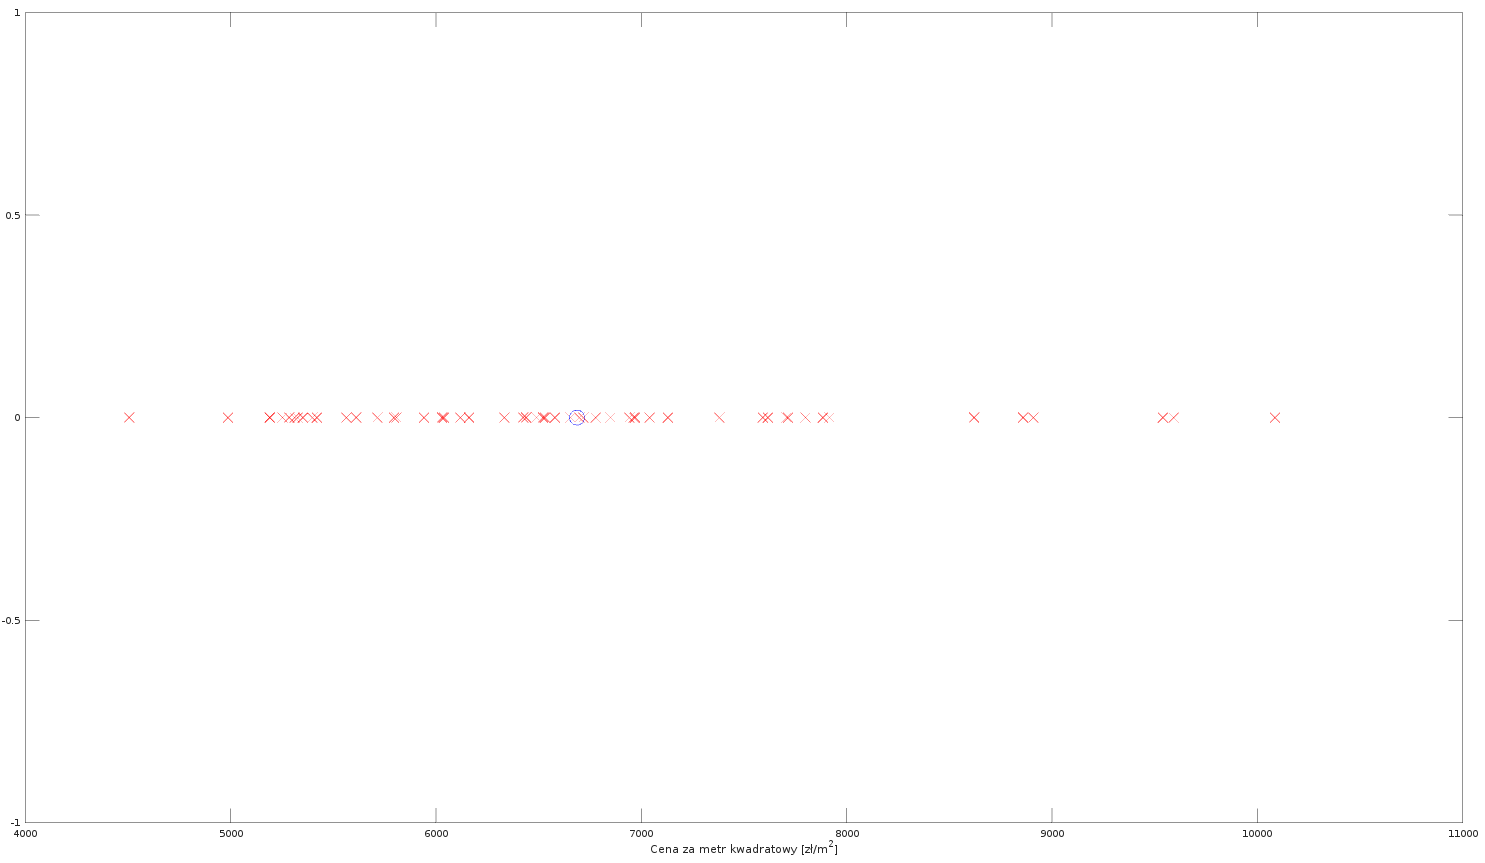
\includegraphics[scale=0.20]{PNG/1D.png}
    \caption{Wykres ceny metra kwadratowego dla wszystkich próbek}
    \label{lamana}
	\end{figure}
	

	\subsection{Dane po filtracji}
	- wykres danych po  \\
	- plusy filtracji \\
	- specyfika filtracji, inne punkty odrzucone niż na pierwszy rzuk oka \\

\end{document}